\section{Auswertung}
\label{sec:Auswertung}

% Fehlerrechnung
Die in diesem Kapitel durchgeführten Fehlerrechnungen wurden mittels der Gaußschen Fehlerfortpflanzung 
\begin{equation}
    \sigma_f = \sqrt{\left( \frac{\partial f}{\partial x_1} \sigma_{x_1} \right)^2 + \left( \frac{\partial f}{\partial x_2} \sigma_{x_2} \right)^2 + ...}
\end{equation}
durchgeführt, sowie den Formeln 
\begin{equation}
    \overline{x} = \frac{1}{n} \sum^n_{i=1}x_i . 
    \label{eq:mittelwert}
\end{equation}
für den Mittelwert und 
\begin{equation}
    \sigma_{\overline{x}} = \frac{\sigma_x}{\sqrt{n}} = \sqrt{\frac{1}{n(n-1)}  \sum^n_{i=1} \left( x_i - \overline{x}\right)^2 } .
    \label{eq:standardabweichung}
\end{equation}
für die Standardabweichung einer Messreihe $\left( x_1, ... , x_n  \right)$.
Der Einfachheit halber wird hierbei das Python-Paket \textit{uncertainties} verwendet. \cite{uncertainties} \\
\hspace{1cm}
% Ende Fehlerrechnung


\subsection{Frequenzabhängigkeit der Leitunsgskonstanten}

Die gemessenen Werte für den Leitungswiderstand $R$, die Induktivität $L$, die Kapazität $C$, die Impedanz $Z$ und die Phasenverschiebung $\varphi$ sind in Tabelle \autoref{tab:RCL} aufgelstet. 

\begin{table}[H]
	\centering
	\caption{Messwerte für Leitungskonstanten $R,L,C,Z,\varphi$ in Abhängigkeit von Frequenz $f$.}
	\label{tab:RCL}
	\begin{tabular}{c | c | c | c | c | c}
		\toprule
		$f \, [\mathrm{kHz}]$ & $R \, [\Omega]$ & $L \, [\mathrm{\mu H}]$ & $C \, [\mathrm{nF}]$ & $Z \, [\Omega]$ & $\varphi \, [°]$\\
		\midrule
		1 & 4,310  \, \clap{$\pm$} \,  0,001 & 25,99  \, \clap{$\pm$} \,  0,01 & 8,530  \, \clap{$\pm$} \,  0,001 & 18660 & -90 \\
		 1,5 & 4,311  \, \clap{$\pm$} \,  0,001 & 25,99  \, \clap{$\pm$} \,  0,01 & 8,530  \, \clap{$\pm$} \,  0,001 & 12440 & -90 \\
		 2 & 4,311  \, \clap{$\pm$} \,  0,001 & 26,00  \, \clap{$\pm$} \,  0,01 & 8,529  \, \clap{$\pm$} \,  0,001 & 9329 & -90 \\
		 2,5 & 4,311  \, \clap{$\pm$} \,  0,001 & 25,97  \, \clap{$\pm$} \,  0,01 & 8,529  \, \clap{$\pm$} \,  0,001 & 7464 & -90 \\
		 3 & 4,312  \, \clap{$\pm$} \,  0,001 & 25,96  \, \clap{$\pm$} \,  0,01 & 8,530  \, \clap{$\pm$} \,  0,001 & 6220 & -90 \\
		 3,5 & 4,312  \, \clap{$\pm$} \,  0,001 & 25,95  \, \clap{$\pm$} \,  0,01 & 8,530  \, \clap{$\pm$} \,  0,001 & 5331 & -90 \\
		 4 & 4,312  \, \clap{$\pm$} \,  0,001 & 25,95  \, \clap{$\pm$} \,  0,01 & 8,530  \, \clap{$\pm$} \,  0,001 & 4665 & -90 \\
		 4,5 & 4,313  \, \clap{$\pm$} \,  0,001 & 25,95  \, \clap{$\pm$} \,  0,01 & 8,529  \, \clap{$\pm$} \,  0,001 & 4146 & -90 \\
		 5 & 4,313  \, \clap{$\pm$} \,  0,001 & 25,95  \, \clap{$\pm$} \,  0,01 & 8,530  \, \clap{$\pm$} \,  0,001 & 3732 & -90 \\
		 5,5 & 4,314  \, \clap{$\pm$} \,  0,001 & 25,95  \, \clap{$\pm$} \,  0,01 & 8,530  \, \clap{$\pm$} \,  0,001 & 3392 & -90 \\
		 6 & 4,314  \, \clap{$\pm$} \,  0,001 & 25,95  \, \clap{$\pm$} \,  0,01 & 8,530  \, \clap{$\pm$} \,  0,001 & 3110 & -90 \\
		 6,5 & 4,315  \, \clap{$\pm$} \,  0,001 & 25,95  \, \clap{$\pm$} \,  0,01 & 8,530  \, \clap{$\pm$} \,  0,001 & 2870 & -90 \\
		 7 & 4,315  \, \clap{$\pm$} \,  0,001 & 25,94  \, \clap{$\pm$} \,  0,01 & 8,530  \, \clap{$\pm$} \,  0,001 & 2665 & -90 \\
		 7,5 & 4,316  \, \clap{$\pm$} \,  0,001 & 25,95  \, \clap{$\pm$} \,  0,01 & 8,530  \, \clap{$\pm$} \,  0,001 & 2488 & -90 \\
		 8 & 4,317  \, \clap{$\pm$} \,  0,001 & 25,95  \, \clap{$\pm$} \,  0,01 & 8,531  \, \clap{$\pm$} \,  0,001 & 2332 & -90 \\
		 8,5 & 4,317  \, \clap{$\pm$} \,  0,001 & 25,95  \, \clap{$\pm$} \,  0,01 & 8,531  \, \clap{$\pm$} \,  0,001 & 2195 & -90 \\
		 9 & 4,318  \, \clap{$\pm$} \,  0,001 & 25,95  \, \clap{$\pm$} \,  0,01 & 8,531  \, \clap{$\pm$} \,  0,001 & 2073 & -90 \\
		 9,5 & 4,319  \, \clap{$\pm$} \,  0,001 & 25,95  \, \clap{$\pm$} \,  0,01 & 8,531  \, \clap{$\pm$} \,  0,001 & 1964 & -90 \\
		 10 & 4,320  \, \clap{$\pm$} \,  0,001 & 25,94  \, \clap{$\pm$} \,  0,01 & 8,531  \, \clap{$\pm$} \,  0,001 & 1866 & -90 \\
		 20 & 4,347  \, \clap{$\pm$} \,  0,001 & 25,93  \, \clap{$\pm$} \,  0,01 & 8,538  \, \clap{$\pm$} \,  0,001 & 932 & -89,9 \\
		 100 & 5,178  \, \clap{$\pm$} \,  0,001 & 26,24  \, \clap{$\pm$} \,  0,01 & 8,781  \, \clap{$\pm$} \,  0,001 & 181,2 & -89,4 \\
		 \bottomrule
	\end{tabular}
\end{table}


Mithilfe der aus \autoref{fig:formel_tabelle} bekannten Formel für den Querleitwertbelag $G$ für ein Koaxialkabel, kann dieser in Abhängigkeit der Frequenz errechnet werden. Für das verwendete Koaxialkabel gelten die Werte~\cite{Durchfuhrung}
\begin{align*}
    d &= \qty{0.9}{\milli\meter} \\
    D &= \qty{2.95}{\milli\meter} \\
    \epsilon_r &= 2.25 \, .
\end{align*}

Damit können $R, L, C$ und $G$ in Abhängigkeit der Frequenz dargestellt werden. Diese Darstellungen sind in \autoref{fig:RCLG} zu sehen.

\begin{figure}[htbp]
    \centering
    \includegraphics[width=\textwidth]{content/plots/RCL.pdf}
    \caption{$R, L, C$ und $G$ in Abhängigkeit der Frequenz $\omega$.~\cite{matplotlib}}
    \label{fig:RCLG}
\end{figure}

\subsection{Dämpfungs- und Dielektrizitätskonstanten}

Für die drei verschiedenen Koaxialkabel mit offenem Ende werden anhand der in \autoref{fig:3kabel_oszi} zu sehenden Oszillogramme des Signalverlaufs die Eingangs- und Reflexionspeaks bestimmt. Außerdem wird die Zeitdifferenz $\Delta t$ zwischen den Peaks vom Oszilloskop abgelesen. \\
Zusätzlich werden für Kabel 1 und Kabel 2 mithilfe eines Zollstocks die Längen $L$ gemessen. Für Kabel 3 wird die Länge als $L \approx \qty{20}{\meter}$ abgeschätzt, da es sich um ein sehr langes Kabel handelt. Die Gültigkeit dieser Abschätzung wird später überprüft. \\

\begin{figure}[htbp]
    \centering
    \begin{subfigure}[b]{0.32\textwidth}
        \centering
        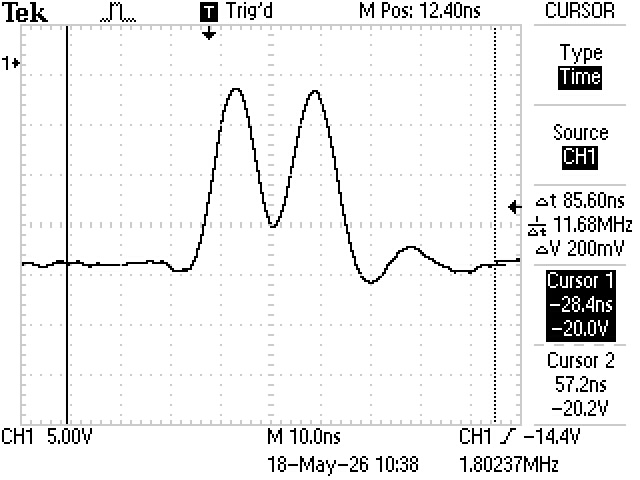
\includegraphics[width=\textwidth]{content/pics/oszi/MittleresKabel.jpg}
        \caption{Kabel 1.}
        \label{fig:kabel1}
    \end{subfigure}%
    \hfill
    \begin{subfigure}[b]{0.32\textwidth}
        \centering
        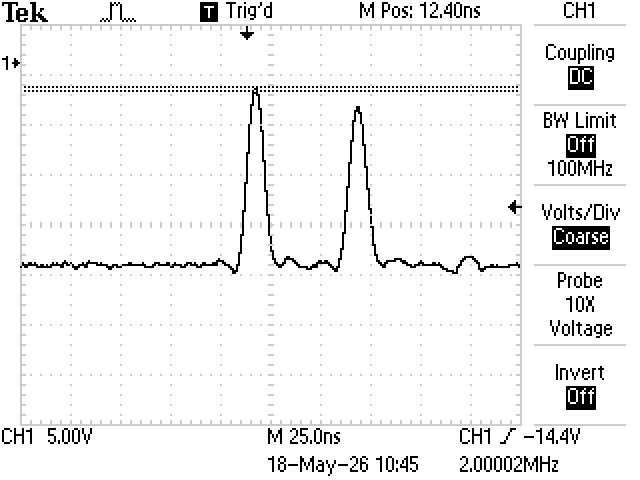
\includegraphics[width=\textwidth]{content/pics/oszi/MittellangesKabel.jpg}
        \caption{Kabel 2.}
        \label{fig:kabel2}
    \end{subfigure}%
    \hfill
    \begin{subfigure}[b]{0.32\textwidth}
        \centering
        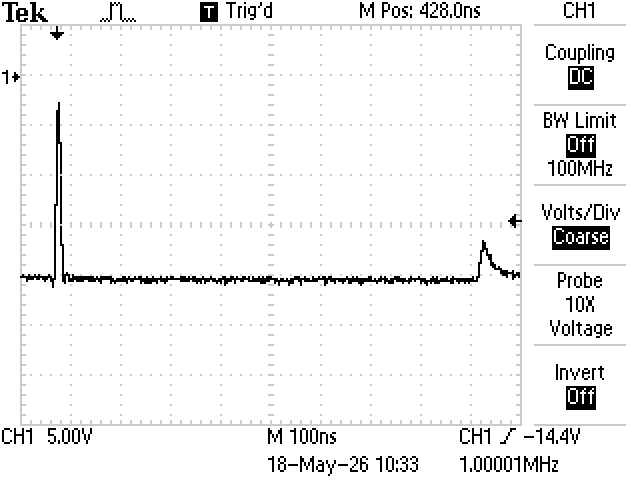
\includegraphics[width=\textwidth]{content/pics/oszi/LangesKabel.jpg}
        \caption{Kabel 3.}
        \label{fig:kabel3}
    \end{subfigure}
    \caption{Oszillogramme der drei Koaxialkabel. Die Eingangs- und Reflexionspeaks sowie die Zeitdifferenz $\Delta t$ sind zu erkennen.}
    \label{fig:3kabel_oszi}
\end{figure}

Die gemessenen Werte für die drei Kabel sind in \autoref{tab:3kabel} aufgelistet.

\begin{table}[h]
\centering
\begin{tabular}{lccccc}
    \toprule
    Kabel & $A_0$ [V] & $A_1$ [V] & Zero-Level [V] & $\Delta t$ [ns] & $L$ [m] \\
    \midrule
    Kabel 1 & -3.2 & -3.52 & -20.2 & 15.6 & 1.5 \pm 0.1 \\
    Kabel 2 & -2.8 & -4.6  & -20.2 & 51.2 & 5.0 \pm 0.5 \\
    Kabel 3 & -2.8 & -15.6 & -19.2 & 856  & 20.0 \\
    \bottomrule
\end{tabular}
\caption{Messwerte für die drei Koaxialkabel. $A_0$ und $A_1$ sind die Spannungen der Eingangs- und Reflexionspeaks, gemessen im Vergleich zum Untergrund-Level (Zero-Level), $\Delta t$ ist die Zeitdifferenz zwischen den Peaks und $L$ ist die Länge des Kabels.}
\label{tab:3kabel}
\end{table}

Anhand der gemessenen Werte können nun die Dämpfungskonstanten $\alpha$ für die jeweiligen Kabel berechnet werden. Dazu wird die Formel \eqref{eq:alpha} verwendet, indem $z=2L$, aufgrund der Hin- nud Rücklaufzeit des Signals, eingesetzt wird. 
$U_0$ und $U(z=2L) := U_1$ werden aus den gemessenen Spannungen als Differenz zum Zero-Level bestimmt, also $U_0 = A_0 - \text{Zero-Level}$ und $U_1 = A_1 - \text{Zero-Level}$. \\
Die umgestellte Formel für $\alpha$ lautet dann 
\begin{equation}
    \alpha = \frac{1}{2L} \ln\left(\frac{U_0}{U_1}\right) .
\end{equation}
Die berechneten Werte für $\alpha$ sind in \autoref{tab:alpha} aufgelistet.

\begin{table}[h!]
\centering
\begin{tabular}{lccccc}
    \toprule
    Kabel & $\alpha$ [1/m] \\
    \midrule
    Kabel 1 & \qty{0.00633(0.00004)}{} \\
    Kabel 2 & \qty{0.0109(0.0001)}{}\\
    Kabel 3 & \qty{0.03791(0.0002)}{} \\
    \bottomrule
\end{tabular}
\caption{Berechnete Dämpfungskonstanten für die drei Koaxialkabel.}
\label{tab:alpha}
\end{table}

\vspace{5cm}
Um nun die Dielektrizitätskonstanten $\epsilon_r$ zu bestimmen wird der bekannte Zusammenhang zwischen der Phasengeschwindigkeit $v_\T{ph}$ und der relativen Dielektrizitätskonstante $\epsilon_r$ verwendet, und nach Länge $L$ und Laufzeit $\Delta t$ umgestellt. Es gilt dann
\begin{align}
    \epsilon_r &= \left( \frac{c}{v_\T{ph}} \right)^2 = \left ( \frac{c \Delta t}{2L} \right)^2 \, ,
\end{align}
wobei $c$ die Lichtgeschwindigkeit im Vakuum ist. Die berechneten Werte für $\epsilon_r$ sind in \autoref{tab:epsilon} aufgelistet.
\begin{table}[h!]
\centering
\begin{tabular}{lccccc}
    \toprule
    Kabel & $\epsilon_r$ \\
    \midrule
    Kabel 1 & \qty{2.43(0.03)}{} \\
    Kabel 2 & \qty{2.36(0.05)}{} \\
    Kabel 3 & \qty{41.16(0.04)}{} \\
    \bottomrule
\end{tabular}
\caption{Berechnete relative Dielektrizitätskonstanten für die drei Koaxialkabel.}
\label{tab:epsilon}
\end{table}

\subsubsection{Gültigkeit der Abschätzung der Länge von Kabel 3}

Es ist zu erkennen, dass die berechnete Dielektrizitätskonstante für Kabel 3 mit einem Wert von $\epsilon_r \approx 41$ deutlich höher liegt als die Werte für Kabel 1 und Kabel 2, die in einem realistischen Bereich von $\epsilon_r \approx 2.4$ liegen. Dies deutet darauf hin, dass die Abschätzung der Länge von Kabel 3 als $L \approx \qty{20}{\meter}$ nicht korrekt ist. \\
Da auch in den meisten handelsüblichen Koaxialkabeln die Dielektrizitätskonstante im Bereich von $\epsilon_r \approx 2$ bis $\epsilon_r \approx 3$ liegt (ohne Quelle), liegt es Nahe, dass die tatsächliche Länge von Kabel 3 deutlich größer als die abgeschätzten $20$ Meter ist. 

Um also die tatsächliche Länge von Kabel 3 zu bestimmen, kann anhand der Messwerte für Kabel 1 und 2 ein Mittelwert für die Phasengeschwindigkeit $v_\T{ph}$, hier mithilfe der Funktion \textit{scipy.stats.linregress}~\cite{scipy}, berechnet werden.\\
Die Lineare Regression liefert die Koeffizienten 
\begin{align}
    m &= \frac{v_\T{ph}}{2} = \qty{0.0983}{\meter\per\nano\second} \\
    b &= \qty{-0.0337}{\meter}
\end{align}
für die Steigung $m$ und y-Achsenabschnitt $b$. \\
Die daraus errechneten Werte für die Länge $L$, Dämpfungskonstante $\alpha$ und  Permeabilität $\epsilon_r$ von Kabel 3 sind 
\begin{align}
    L_\T{K3, estimated} &= \qty{84.16}{\meter} \\
    \alpha_\T{K3, estimated} &= \qty{0.009}{\per\meter} \\
    {\epsilon_r}_\T{K3, estimated} &= 2.32 \; .
\end{align}

Ein Vergleich der Werte für verschiedene Längen $L$ von Kabel 3 ist, zusammen mit der linearen Regression, in \autoref{fig:real_l} zu sehen.

\begin{figure}[htbp]
    \centering
    \includegraphics[width=0.8\textwidth]{content/plots/vphase.pdf}
    \caption{Vergleich der gemessenen Daten mit Annahme $L_\T{K3} \approx 20 \mathrm{m}$ und anhand der anderen Werte abgeleiteten Länge $L_\T{K3} \approx 80 \mathrm{m}$.}
    \label{fig:real_l}
\end{figure}



\subsection{Abschlüsse}




\clearpage